\documentclass[a5paper]{ufsc-thesis}  % escolha o tamanho do papel aqui

% Gerador de texto
\usepackage{lipsum}
\usepackage{array}
\newcolumntype{P}[1]{>{\centering\arraybackslash}p{#1}}
\newcolumntype{M}[1]{>{\centering\arraybackslash}m{#1}}

\usepackage{times}
\usepackage{cmap}
\usepackage[utf8]{inputenc}
\usepackage[T1]{fontenc}

\usepackage{indentfirst}		% Indenta o primeiro parágrafo de cada seção.
\usepackage{color}				% Controle das cores
\usepackage{graphicx}			% Inclusão de gráficos
\usepackage{microtype} 			% para melhorias de justificação
\usepackage{amsmath} 			% para melhorias de justificação

\usepackage[brazilian,hyperpageref]{backref}	  % Paginas com as citações na bibl
\usepackage[alf]{abntex2cite}	                  % Citações padrão ABNT
\usepackage[left=2.5cm, right=1.5cm, top=2cm, bottom=1.5cm]{geometry}

\usepackage{titlesec}
\usepackage{longtable}
\usepackage{subcaption}

\usepackage{listings}
\usepackage[final]{pdfpages}

\usepackage[backend=biber,style=alphabetic,sorting=ynt]{biblatex}
\addbibresource{mybibliography.bib}

% ---
% Informações de dados para CAPA e FOLHA DE ROSTO
% ---
\titulo{Uma Análise da Eficiência Energética do Processamento em um Dispositivo IoT versus Processamento em um Servidor}
\autor{Guilherme Henrique Paggi Daros}
\local{Florianópolis}
\data{2024}
\orientador{Richard Demo Souza}
\coorientador{Elço João dos Santos Júnior}
\instituicao{Universidade Federal de Santa Catarina - UFSC}
\programa{Graduação em Engenharia Eletrônica}
\tipotrabalho{Trabalho de Conclusão de Curso (graduação)}
% O preambulo deve conter o tipo do trabalho, o objetivo, 
% o nome da instituição e a área de concentração 
\preambulo{Trabalho de Conclusão de Curso submetido ao Departamento de Engenharia Elétrica e Eletrônica da Universidade Federal de Santa Catarina para a obtenção do título de Bacharel em Engenharia Eletrônica.}

% Preâmbulo
\centro{Centro Tecnológico - CTC}
\assuntos{Engenharia Eletrônica, Comunicações Sem Fio, BLE, Machine Learning, Tensorflow Lite}

\titleformat{\section}{%
    \normalfont%
}{\thesection}{1em}{\MakeUppercase}

\begin{document}

% Inicia parte pré-textual do documento capa, folha de rosto, folha de
% aprovação, aprovação, resumo, lista de tabelas, lista de figuras, etc.
\pretextual%
\imprimircapa%
\imprimirfolhaderosto*%
\clearpage

\includepdf{ficha-cat.pdf}
% \imprimirfichacatalografica

% ---
% Inserir folha de aprovação
% ---

% Isto é um exemplo de Folha de aprovação, elemento obrigatório da NBR
% 14724/2011 (seção 4.2.1.3). Você pode utilizar este modelo até a aprovação
% do trabalho. Após isso, substitua todo o conteúdo deste arquivo por uma
% imagem da página assinada pela banca com o comando abaixo:

\begin{folhadeaprovacao}

 \begin{center}
   {\ABNTEXchapterfont\large\imprimirautor}

   \vspace*{\fill}
   \begin{center}
     \ABNTEXchapterfont\bfseries\Large\imprimirtitulo
   \end{center}
   \vspace*{\fill}
   
 Este Trabalho foi julgado adequado para obtenção do Título de Bacharel em Engenharia Eletrônica e aprovado em sua forma  pela sua Banca Examinadora.\\
  \imprimirlocal, 20 de fevereiro de \imprimirdata.
   
  \end{center}
   
  \assinatura{\textbf{Prof. Daniela Ota Hisayasu Suzuki, Dr.} \\ Coordenadora do Curso\\~\\} 
   
  \textbf{Banca examinadora:}
  \vspace*{\fill}
  \assinatura{\textbf{Prof. \imprimirorientador, Dr.} \\ Orientador \\ Universidade Federal de Santa Catarina\\}\vspace*{\fill}
  \assinatura{\textbf{Prof. Glauber Gomes de Oliveira Brante, Dr.} \\ Universidade Tecnológica Federal do Paraná\\}
  \vspace*{\fill}
  \assinatura{\textbf{Prof. Walter Pereira Carpes Junior, Dr.} \\ Universidade Federal de Santa Catarina\\}   
\end{folhadeaprovacao}
% ---

% ---
% Dedicatória
% ---
\begin{dedicatoria}
   \vspace*{\fill}
	\begin{flushright}
		\textit{"Este trabalho é dedicado à meus familiares e amigos que me acompanharam nesta jornada. Sem o seu apoio não teria chegado até aqui."}
	\end{flushright}
\end{dedicatoria}
% ---

% ---
% Agradecimentos
% ---
\begin{agradecimentos}
Agradeço primeiramente minha família, na figura dos meus pais, Sara e Fernando, pelo apoio durante toda minha vida e principalmente nestes anos de faculdade.

Agradeço também aos meus amigos de longa data, Rafael Tapajóz, Luiz Felipe Vigana, João Guilherme, Victor Guerreiro, Victor Hugo da Silva, Lucas Machado e Leonardo Becker por, mesmo de longe, sempre me incentivarem a buscar meus objetivos pessoais e profissionais.

Não poderia deixar de agradecer aos meus amigos de Florianópolis, Leonardo Renz, Silney de Aquino, Jorge Delfino, Daniel Zaiden, por me acompanharem de perto nessa trajetória universitária.

Agradeço a todos os colegas de curso e departamento que estiveram presentes diariamente durante esta trajetória, em especial meus amigos e colegas de turma Andrio Souza e Luís Piva.

Agradeço ao meu orientador e professor, Richard Demo Souza, pelos aprendizados nas disciplinas cursadas e pela orientação deste trabalho, e também ao meu coorientador Elço João dos Santos Júnior, pelo suporte na realização dos testes necessários.

Agradeço também a equipe Vento Sul - Barco Solar UFSC, por todas as oportunidades de aprendizado nos dois anos e meio que participei, ao Instituto de Eletrônica de Potência, pela oportunidade de Iniciação Científica, que certamente contribuiu para minha formação como engenheiro, e a Fundação Certi, empresa na qual fiz meu estágio obrigatório e onde, com meus colegas de trabalho, aprendi muito sobre o mercado e sobre a carreira que escolhi seguir.

Agradeço a todos os servidores e técnicos do Departamento de Engenharia Elétrica e Eletrônica por trabalharem diariamente para tornar possível este momento para mim e para todos os outros estudantes.

Por fim agradeço a mim mesmo, por mesmo nos momentos difíceis e conturbados inerentes a graduação ter mantido o foco no objetivo, me tornar um engenheiro eletrônico.
\end{agradecimentos}
% ---

% ---
% Epígrafe
% ---
\begin{epigrafe}
    \vspace*{\fill}
	\begin{flushright}
		\textit{``Tu te tornas eternamente responsável por aquilo que cativas"\\
		(Saint-Exupéry, Antoine de; O Pequeno Príncipe, 1952)}
	\end{flushright}
\end{epigrafe}
% ---

% ---
% RESUMOS
% ---

% resumo em português
\setlength{\absparsep}{18pt} % ajusta o espaçamento dos parágrafos do resumo

\begin{resumo}
 \noindent O trabalho em questão aborda uma comparação entre duas arquiteturas de aplicações de sensoriamento. Utiliza-se como base um dispositivo alimentado a bateria, que coleta dados de sensores e os transmite para um servidor central, no qual algoritmos de aprendizado de máquina processam estes dados para tomada de decisão. Sabendo que transmissões de dados utilizando tecnologias sem fio possuem custo energético elevado, este trabalho estuda os efeitos da transferência destes algoritmos para o dispositivo na borda, minimizando a quantidade de transmissões realizadas visando aumentar a eficiência energética. Para este comparativo são utilizados o Bluetooth Low Energy como tecnologia de comunicação sem fio e o TensorFlow Lite Micro como biblioteca de aprendizado de máquina. 
 
 \vspace{\onelineskip}
 
 \noindent \textbf{Palavras-chave}: comunicações sem fio. aprendizado de máquina. bluetooth low energy.
 \end{resumo}

% resumo em inglês

\begin{resumo}[Abstract]
 \begin{otherlanguage*}{english}
   \noindent This work addresses a comparison between two sensing application architectures. A battery powered device collects data and transmits it to a central service, in which machine learning algorithms are used to process this inputs and make decisions. Knowing that data transmission using wireless technologies has a high energy cost, this work studies the transfer of these algorithms to the edge device, minimizing the amount of transmissions, targeting the improvement of energy efficiency. In this comparison Bluetooth Low Energy is used as wireless technology and the TensorFlow Lite Micro as machine learning library.

   \vspace{\onelineskip}
 
   \noindent 
   \textbf{Keywords}: wireless communication. machine learning. bluetooth low energy.
 \end{otherlanguage*}
\end{resumo}


% ---
% inserir lista de ilustrações
% ---
\renewcommand*\listfigurename{Lista de figuras}
\pdfbookmark[0]{\listfigurename}{lof}
\listoffigures*
\cleardoublepage
% ---

% ---
% inserir lista de tabelas
% ---
\pdfbookmark[0]{\listtablename}{lot}
\listoftables*
\cleardoublepage
% ---

% ---
% inserir o sumario
% ---
\pdfbookmark[0]{\contentsname}{toc}
\tableofcontents*
\cleardoublepage
% ---


% ----------------------------------------------------------
% ELEMENTOS TEXTUAIS
% ----------------------------------------------------------
\textual

% ---
% Introdução [WIP]
% ---
\chapter{Introdução}

Segundo uma pesquisa da IC Insights, existem mais de 250 bilhões de microcontroladores no mundo \cite{ic_insights}, com grande potencial de crescimento no próximos anos. Neste contexto, aplicações de sensoriamento tem ganhado um papel importante em diversas áreas como saúde, monitoramento ambiental e manutenção preventiva. Tais aplicações usualmente são constituídas por dispositivos alimentados por baterias que coletam e transmitem dados para um servidor para análise e tomada de decisão. Porém, restrições inerentes a estes tipos de dispositivos impõem desafios significativos de eficiência energética e sustentabilidade destes sistemas, sendo particularmente acentuados em cenários nos quais transmissão de dados sem fio é necessária.

A eficiência energética dos dispositivos de Internet das Coisas, em inglês Internet of Things (IoT), não é apenas um desafio técnico, mas uma questão importante tanto para sustentabilidade ambiental quanto viabilidade econômica destas tecnologias. Acompanhando a necessidade do mercado, o Bluetooth Low Energy (BLE) surge como uma alternativa interessante. Nascido da visão do Bluetooth Special Interest Group (Bluetooth SIG) de otimizar a conectividade para aplicações de baixo consumo e curto alcance \cite{Townsend_2014}, o BLE rapidamente se tornou importante no campo de IoT, alimentando uma vasta gama de dispositivos, desde vestíveis e \textit{gadgets} de saúde até casas inteligentes e sensores industriais.

Sabendo que transmissões de dados sem fio são potencialmente a tarefa com maior custo energético executada por dispositivos IoT, este trabalho estuda o uso de técnicas de aprendizado de máquina embarcadas para minimizar a necessidade de transmitir muitos dados para um servidor, atingindo maior eficiência energética.

Uma aplicação que se encaixa neste contexto é o uso de dados de acelerômetro preso ao corpo de uma pessoa para realizar classificação de atividade humana, como caminhando, subindo escadas, caminhando enquanto conversa com outra pessoa, como descrito em \cite{hyerarchical_ML}.

Para tal é utilizada uma aplicação base como ponto de partida, que possui o seguinte fluxo de execução, que é típico de muitas aplicações IoT \cite{survey_ml_for_iot}:
\begin{itemize}
    \itemsep-0.5em
    \item Dispositivo em modo low power, processador e rádio desligados;
    \item Processador é acordado por um temporizador externo, via interrupção;
    \item Processador liga a alimentação de um acelerômetro e faz a leitura do mesmo;
    \item Processador liga o rádio e transmite os dados coletados;
    \item Processador desliga tanto acelerômetro quanto rádio;
    \item Processador configura o temporizador externo;
    \item Processador se desliga, colocando o dispositivo em modo low power e o ciclo se repete.
\end{itemize}

Uma representação gráfica do fluxo de execução da aplicação base pode ser vista na Figura \ref{fig:base_app}.
\begin{figure}[!ht]
    \centering
    \includegraphics[width=0.8\linewidth]{imagens/base_app.eps}
    \caption{Fluxo de execução da aplicação base, fonte: autor}
    \label{fig:base_app}
\end{figure}

Por sua vez, a aplicação proposta, utilizando um modelo de aprendizado de máquina baseado em rede neural, processa os dados no dispositivo IoT transmitindo apenas o resultado deste processamento. Assim, há uma redução tanto no volume bruto de dados transmitidos para o servidor central quanto na quantidade de transmissões necessárias para o funcionamento da aplicação. Como transmissões em redes sem fio tendem a consumir uma quantidade significativa de energia, reduzir a frequência com a qual a aplicação precisa transmitir pode aumentar significativamente a sua eficiência energética.

Assim, a aplicação proposta segue o seguinte fluxo de execução:

\begin{itemize}
    \itemsep-0.5em 
    \item Dispositivo em modo low power, processador e rádio desligados;
    \item Processador é acordado por temporizador externo, via interrupção;
    \item Processador liga a alimentação de um acelerômetro e faz a leitura do mesmo;
    \item Processador salva em memória persistente os dados lidos;
    \item Processador se desliga, colocando o dispositivo em modo low power e este ciclo é repetido $M-1$ vezes;
    \item Na $M$-ésima execução os dados são recuperados da memória persistente;
    \item Dados são pré-processados, extraindo atributos dos mesmos;
    \item Atributos são fornecidos como entrada para o modelo de aprendizado de máquina;
    \item Modelo é executado e seu resultado lido;
    \item Processador liga o rádio e transmite o resultado;
    \item Processador desliga tanto acelerômetro quanto rádio;
    \item Processador configura o temporizador externo;
    \item Processador se desliga, colocando o dispositivo em modo low power e o ciclo completo se repete.
\end{itemize}

Uma representação gráfica do fluxo de execução da aplicação proposta pode ser vista na Figura \ref{fig:prop_app}.

\begin{figure}[!ht]
    \centering
    \includegraphics[width=0.8\linewidth]{imagens/prop_app.eps}
    \caption{Fluxo de execução da aplicação proposta, fonte: autor}
    \label{fig:prop_app}
\end{figure}

\section{Objetivos}
A seguir estão destacados os objetivos deste trabalho de conclusão de curso, separados em objetivos gerais e objetivos específicos.

\subsection{Objetivo geral}
Realizar uma comparação de consumo energético entre duas aplicações de IoT, uma aplicação base, com processamento no servidor, e a aplicação proposta, que realiza processamento local, com vistas a compreender em quais casos há melhora significativa de eficiência energética.
\subsection{Objetivos específicos}
De maneira específica, os objetivos deste trabalho  são:
\begin{itemize}
    \item Estudar o padrão BLE, desenvolvido e comercializado pelo Bluetooth SIG;
    \item Estudar a biblioteca de aprendizado de máquina embarcado TensorFlow Lite Micro (TFLM), desenvolvido pela Google e publicado sob a licença de software livre Apache 2.0;
    \item Construir aplicações de IoT e inferência baseado em aprendizado de máquina utilizando as tecnologias citadas acima;
    \item Realizar testes e adquirir dados de consumo energético das aplicações construídas;
    \item Analisar a viabilidade deste tipo de técnica variando-se parâmetros relacionados à aplicação proposta.
\end{itemize}

\section{Delimitações}
Não faz parte do objetivo deste trabalho analisar os modelos de aprendizado de máquina utilizados quanto a sua assertividade na tarefa desempenhada, mas somente avaliar as aplicações de um ponto de vista de consumo energético.

\section{Estrutura do Trabalho}

A estrutura do trabalho foi dividida em sete capítulos, que são individualmente explicados nos parágrafos que seguem.

O Capítulo 1, Introdução, tem como objetivo contextualizar e justificar o trabalho, trazendo consigo os objetivos a serem cumpridos, bem como as delimitações e a estrutura em que ele foi montado.

No Capítulo 2, Aprendizado de Máquina, são apresentados os principais desafios encontrados no uso de aprendizado de máquina em aplicações embarcadas, o fluxo de trabalho  no ecossistema do TensorFlow e por fim detalhamentos sobre o TFLM como sua implementação de interpretador, gerenciamento dinâmico de memória, suporte a operações matemáticas comuns e seu suporte a diferentes hardwares.

No Capítulo 3, Bluetooth Low Energy, é feito um panorama geral sobre o padrão BLE passando pela base do protocolo separada em camada física e camada de enlace de dados, além das estruturas e procedimentos presentes em camadas mais altas da \textit{stack} do BLE.

No Capítulo 4, Hardware e Firmware, apresenta-se os dispositivos de hardware, as ferramentas de software e a estrutura do projeto utilizados nos testes.

No Capítulo 5, Testes, descreve-se o modelamento matemático do consumo energético das aplicações, os equipamentos e o ambiente utilizados nos testes, incluindo também uma descrição dos dados adquiridos e condições de medição.

No Capítulo 6, Resultados, são expostos o desenvolvimento dos modelos de trabalho do dispositivo de IoT, bem como os métodos e processos utilizados para se atingir os objetivos inicialmente previstos no Capítulo 1.

No Capítulo 7, Conclusões e Recomendações, são descritos e discutidos os resultados obtidos, realizando correlações com os objetivos que nortearam a execução deste trabalho. Também são realizadas algumas proposições para estudos futuros.

% ---
% TFLite Micro [ FEITO, REVISADO ]
% ---
\chapter{Aprendizado de Máquina}

Tratando-se de uma tarefa de aprendizado de máquina supervisionado, o fluxo de trabalho usualmente consiste numa etapa de treinamento, executada em dispositivos com amplo poder computacional e acesso a grandes conjuntos de dados, e numa etapa de inferência \cite{Danilo22}, que requer menos recursos e portanto pode ser executada em dispositivos mais simples, como sistemas embarcados. 

O TFLM é uma biblioteca de inferência de aprendizado de máquina de código aberto projetado para executar modelos de aprendizado profundo em sistemas embarcados \cite{tflu}. O TFLM aborda as demandas de eficiência impostas pelas restrições de recursos inerentes aos sistemas embarcados e os desafios da fragmentação do mercado que dificultam a interoperabilidade entre processadores de diferentes fabricantes. Para tal, o TFLM é implementado com base em um interpretador, oferecendo tanto flexibilidade de uso do ponto de vista de aplicação, quanto lidando com as restrições já citadas.

Como dito anteriormente o TFLM é uma biblioteca apenas de inferência, portanto a etapa de treinamento é realizada utilizando outra ferramenta, do mesmo ecossistema, o próprio TensorFlow e sua API de alto nível, o Keras. Com isso o fluxo de trabalho no desenvolvimento, construção e treinamento de novos modelos de aprendizado profundo pode ser realizado independente de plataforma alvo e utilizando ferramentas consolidadas e bastante conhecidas no mercado de inteligência artificial. Este capítulo traz uma breve introdução sobre a arquitetura do TFLM.

\section{Arquitetura}

\begin{figure}[!ht]
    \centering
    \includegraphics[width=0.8\linewidth]{imagens/tflm_arch.eps}
    \caption{Arquitetura do TensorFlow Lite Micro, adaptado de \cite{tflu}}
    \label{fig:tflm_arch}
\end{figure}

A arquitetura proposta e implementada pelo TFLM é composta por diversos agentes como pode ser visto na Figura \ref{fig:tflm_arch}, cada um responsável por uma tarefa específica:
\begin{itemize}
    \item \textit{Operation Resolver}: Mapeia as operações descritas no fluxo de execução do modelo para suas implementações, que podem ou não ser dependentes de hardware;
    
    \item \textit{Model Loader}: Responsável por ler o modelo em formato Flatbuffer, armazenado em memória não volátil, e criar uma representação deste em memória RAM, contendo informações sobre as entradas, o fluxo de execução e as saídas;
    
     \item \textit{Memory Planner}: A ausência de alocação dinâmica de memória implicaria em reservar memória específica para cada operação necessária em tempo de compilação, sendo que muitas operações necessitariam de muita memória. Como memória é um recurso escasso em sistemas embarcados, o compilador reserva uma região e passa o controle total para o interpretador, que, em tempo de execução, implementa um algoritmo de planejamento de uso de memória.
\end{itemize}


\section{Interpretador}
    Como dito anteriormente, o TFLM é baseado em um interpretador que lida, em tempo de execução, com os modelos de aprendizado de máquina passados para ele. Diferentemente de execução estática de código, o interpretador tem acesso a uma estrutura de dados que define completamente o modelo, possibilitando controle sobre as operações e parâmetros em tempo de execução.
    
    Esta abordagem foi escolhida baseada em experiências do dia a dia com sistemas embarcados \cite{tflu}, dando ênfase na facilidade de troca de modelos em campo, compartilhamento de código entre diversas aplicações e manutenção simplificada, possibilitando atualizações do modelo sem a necessidade de compilar todo o código fonte novamente. A eficiência do interpretador vem da complexidade natural da execução de modelos, tornando o tempo de execução do interpretador por si só quase desprezível em relação às operações de álgebra linear que o modelo necessita. Além disto, com a visão de suportar a maior gama possível de processadores e arquiteturas, o TFLM não utiliza nenhuma biblioteca pré-compilada, tornando a jornada da ideia até uma aplicação funcional bastante acessível.
   
\section{Modelo}
    O interpretador em questão utiliza uma estrutura de dados que define por completo um modelo de aprendizado de máquina utilizando a mesma estrutura do TensorFlow Lite, o FlatBuffer. Apesar de ocupar pouca memória, essa biblioteca depende da especificação C++11 do compilador da plataforma alvo, exigindo colaboração com fabricantes de processadores para atualizar suas ferramentas visto que no âmbito de sistemas embarcados é comum utilizar especificações bastante antigas. O formato Flatbuffer foi inicialmente projetado para dispositivos com sistema de arquivo, houve um certo desafio com dispositivos que não possuem esta funcionalidade \cite{tflu}, situação comum na área de embarcados, porém a representação serializada facilitou a conversão para arquivos fonte em linguagem C contendo matrizes de dados, que podem então ser compilados no binário para referência fácil da aplicação.
    % Referencia a seção 4.3.1, segundo paragrafo

    A representação do modelo em memória é implementada como uma lista de operações ordenadas topologicamente, vindo de um grafo acíclico direto, o que garante que o tempo de busca de uma operação é linear. Como a geração desta lista acontece em tempo de exportação do modelo, isto não incorre em uso excessivo de recursos pelo interpretador

\section{Gerenciamento de Memória}
    O TFLM adota uma estratégia de gerenciamento de memória baseada em uma arena, espaço contínuo de memória. Durante a fase de preparação do modelo, seu interpretador realiza um planejamento de memória, considerando os tempos de vida e tamanho dos tensores em tempo de execução, memória persistente, metadados do modelo e memória temporária para retenção de dados durante a execução da inferência.

    Com base nos tempos de vida e tamanho dos buffers necessários para cada tarefa, conjuntamente com o tamanho total da arena, o interpretador gera um plano de alocação de memória baseado em um algoritmo conhecido como \textit{First Fit Decreasing}, que possui baixa complexidade e fornece resultados suficientemente bons.

\begin{figure}[h]
    \centering
    \includegraphics[width=0.8\linewidth]{imagens/first_fit_mem_alloc.eps}
    \caption{Esquemas de alocação de memória, adaptado de \cite{tflu}}
    \label{fig:first_fit_mem_alloc}
\end{figure}

\section{Operadores}
No contexto do TFLM, um operador é uma função com parâmetros de entrada e de saída bem definidos, além de um estado interno também pré-definido. A implementação das operações matemáticas do operador pode ser realizada de diversas maneiras, possibilitando que cada fabricante de hardware implemente cada operador para usar de forma ótima o hardware que fornecem. Durante o desenvolvimento da biblioteca em questão, houve colaboração próxima do time do Google e das fornecedoras de tecnologia de processador Arm, Synopsis, Cadence entre outras. Um exemplo é a biblioteca CMSIS-NN \cite{cmsis_nn}, que implementa, de forma otimizada, suporte a operações como convolução, função de ativação RELU, multiplicação de matrizes para processadores com arquitetura ARM.

% ---
% BLE [ FEITO, REVISADO ]
% ---
\chapter{Bluetooth Low Energy}

\section{Camada Física}

A camada física do BLE é o meio pelo qual dados são convertidos em ondas eletromagnéticas que se propagam entre dispositivos, carregando consigo informações que podem ser decodificadas para recuperar os dados originais \cite{Tanenbaum_Wetherall_2014}. 
Um rádio BLE utiliza parte da banda de frequência industrial, científica e médica, em torno de 2.4GHz \cite{Townsend_2014}. Esta banda é divida em 40 canais de mesma largura de banda entre 2.4000 GHz a 2.4835 GHz. Como pode ser visto na Figura \ref{fig:ble_channels}, os primeiros 37 canais são utilizados para comunicação enquanto os últimos três são utilizados para negociar conexões e enviar dados em \textit{broadcast}.
Para lidar com interferência entre dispositivos o padrão BLE adota uma técnica chamada \textit{Frequency Hopping Spread Spectrum}, na qual para cada transmissão, em uma conexão estabelecida, um canal diferente é utilizado \cite{Tanenbaum_Wetherall_2014}, sendo este determinado como:

\begin{figure}
    \centering
    \includegraphics[width=1\linewidth]{imagens/ble_channels.eps}
    \caption{Distribuição dos canais do BLE, adaptado de \cite{Townsend_2014}}
    \label{fig:ble_channels}
\end{figure}

\begin{equation}
    \text{next\_channel = (current\_channel + hop) mod 37}.
\end{equation}

O parâmetro hop é negociado entre os dispositivos no estabelecimento da conexão. A modulação utilizada para codificar os bits em ondas eletromagnéticas é a \textit{Gaussian Frequency Shift Keying} e possui taxa de 1 Mbit/s.

\section{Camada de Enlace de Dados}
A camada de enlace de dados é responsável por definir as janelas de transmissão e gerar as sequências de bits a serem moduladas na camada física \cite{Tanenbaum_Wetherall_2014}. É nesta camada que os requisitos de temporização definidos pela normatização do BLE devem ser atendidos, portanto esta é usualmente implementada com hardware e software específicos, além de ser isolada das camadas superiores por uma padrão de comunicação nomeado \textit{Host Controller Interface} (HCI) \cite{Townsend_2014}. 
Tarefas computacionalmente complexas e de fácil automação são tipicamente implementadas diretamente em silício, das quais podem ser citadas:

\begin{itemize}
    \item Cálculo e verificação de CRC;
    \item Encriptação AES;
    \item Geração de preâmbulo e endereço de acesso.
\end{itemize}

A porção de software desta camada gerencia o estado do rádio e das conexões ativas no momento. É também na camada de enlace que os papéis dos dispositivos são definidos. Dispositivos que iniciam conexões são nomeados como \textit{master} e dispositivos que realizam \textit{advertising} são nomeados \textit{slave}. Existe uma assimetria nos papéis desempenhados pois são necessários mais recursos para agir como \textit{master} do que como \textit{slave}. Isto torna possível que periféricos utilizem componentes mais simples e consequentemente mais baratos, delegando a tarefas de maior complexidade para dispositivos com mais recursos, como notebooks e smartphones.

\subsection{\textit{Bluetooth Device Address}}
Em redes sem fio o meio de propagação de informações é compartilhado, portanto existe a necessidade de um acordo prévio em como o acesso ao meio será realizado \cite{Goldsmith_2020}. Para garantia de identificação de mensagens e de forma semelhante ao \textit{Ethernet Media Access Control (MAC) address}, no Bluetooth é utilizado um número que identifica unicamente cada dispositivo. Este número é um inteiro não sinalizado de 48 bits (6 bytes) que pode pertencer a uma de duas categorias, como descrito em \cite{Townsend_2014}:

\begin{itemize}
    \item \textit{Public device address}: valor fixo, programado em fábrica, deve ser registrado juntamente à \textit{IEEE Registration Authority} e nunca irá mudar durante o tempo de vida do dispositivo;
    \item \textit{Random device address}: utilizado quando o fabricante não quer ou não precisa de registro com a IEEE, podendo ser gerado tanto durante fabricação quanto a cada vez que o dispositivo é energizado. Também há a possibilidade de gerar um novo endereço de tempos em tempos, de acordo com uma chave previamente distribuída, sendo esta parte do padrão implementada quando há necessidade de uma comunicação muito segura.
\end{itemize}


\subsection{Pacotes BLE}
No contexto do BLE existem apenas dois tipos de pacotes: \textit{advertising packets} com os quais é realizado o processo de descobrimento e conexão, além de transmissão de dados em \textit{broadcast}, e \textit{data packets}, trocados após o estabelecimento de uma conexão \cite{Townsend_2014}.

\begin{figure}[h]
    \centering
    \includegraphics[width=1\linewidth]{imagens/ble_packet.eps}
    \caption{Representação visual de um pacote BLE, adaptado de \cite{nordic_semi_academy}}
    \label{fig:ble_packet}
\end{figure}

% PAGINA 2673 da core spec 5.3
Um pacote BLE é composto por um preâmbulo, utilizado para sincronizar as portadoras dos rádios envolvidos, um endereço de acesso, que possui valor fixo para \textit{advertising packets} \cite{bt_core}, \texttt{0x8E89BED6}, a unidade de dados do protocolo, cujo conteúdo depende do tipo de pacote, e por fim um CRC, calculado sobre o restante dos bits e responsável por garantir a integridade do pacote. Uma representação de um pacote BLE pode ser vista na Figura \ref{fig:ble_packet}.

A unidade de dados do protocolo para \textit{advertising packets} é composta por dois bytes de \textit{header} e um \textit{payload} de até 37 bytes, destes, os primeiros seis bytes são dedicados ao \textit{Bluetooth Device Address}, restando 31 bytes para dados de usuário. A estrutura da unidade de dados do protocolo pode ser vista na Figura \ref{fig:ble_adv_packet}. 

\begin{figure}[h]
    \centering
    \includegraphics[width=1\linewidth]{imagens/ble_adv_pdu.eps}
    \caption{Estrutura da unidade de dados de protocolo para \textit{advertising packet}, adaptado de \cite{nordic_semi_academy}}
    \label{fig:ble_adv_packet}
\end{figure}

O \textit{header} carrega consigo três características essenciais para o protocolo, são elas:
\begin{itemize}
    \item Capacidade de conexão\begin{itemize}
        \item Conectável: um dispositivo central pode iniciar o processo de conexão com este periférico;
        \item Não Conectável: um dispositivo central não pode iniciar uma conexão com este periférico, é utilizado somente para transmissão de dados em \textit{broadcast};
    \end{itemize}
    
    \item Escaneabilidade\begin{itemize}
        \item Escaneável: um dispositivo central pode emitir um \textit{scan request} para este periférico após receber um \textit{advertising packet};
        \item Não Escaneável: um dispositivo central não pode emitir um \textit{scan request} para este periférico após receber um \textit{advertising packet};
    \end{itemize}

    \item Diretividade\begin{itemize}
        \item Direcionado: contém apenas os endereços dos dispositivos periférico e central, dados de usuário não são permitidos. É utilizado no reestabelecimento de uma conexão;
        \item Não direcionado: contém o endereço do dispositivo alvo e pode conter dados de usuário.
    \end{itemize}
\end{itemize}

Os dados de \textit{advertising} de um \textit{advertising packet} são separados em campos, cada campo conta com um byte que determina o seu comprimento, um byte responsável por identificar o tipo de dado contido, e um ou mais bytes que representam os dados contidos no campo. Uma descrição visual pode ser vista na Figura \ref{fig:ble_adv_data}

\begin{figure}[h]
    \centering
    \includegraphics[width=1\linewidth]{imagens/ble_adv_data.eps}
    \caption{Estrutura dos dados para \textit{advertising packet}, adaptado de \cite{nordic_semi_academy}}
    \label{fig:ble_adv_data}
\end{figure}

% PAGINA 2746 da core spec 5.3
 \textit{Advertising packets} são utilizados para duas finalidades, descobrimento de um periférico por um dispositivos central e transmissão de dados em \textit{broadcast}. Podem ser transmitidos sem necessidade de resposta ou da existência prévia de um dispositivo para receber. Seu intervalo de transmissão é especificado em norma, \cite{bt_core}, e pode variar de 20 milissegundos a 10485 segundos, seguindo múltiplos de 0.625 milissegundos, oferendo uma ampla faixa de valores que podem ser escolhidos para balancear consumo de energia e chance de descobrimento por outro dispositivo.

\subsection{Descobrimento}
O processo de descobrimento, ilustrado na Figura \ref{fig:ble_discover}, envolve no mínimo dois dispositivos, um atuando como periférico e transmitindo \textit{advertising packets} em \textit{broadcast} e outro atuando como central e escaneando de forma intervalada os três canais dedicados ao \textit{advertising}. Quando ocorre sobreposição entre os intervalos o processo de descobrimento está realizado. A norma prevê a possibilidade de o dispositivo central emitir \textit{scan request} direcionado ao periférico para solicitar mais um pacote com informações extras antes de solicitar uma conexão.

\begin{figure}[h]
    \centering
    \includegraphics[width=1\linewidth]{imagens/ble_discover.png}
    \caption{Processo de descobrimento BLE, fonte \cite{Townsend_2014}}
    \label{fig:ble_discover}
\end{figure}


\subsection{Conexões}
% PAGINA 2790 da core spec 5.3
Uma conexão nada mais é que uma sequência de eventos nos quais \textit{data packets} são trocados entre um dispositivo periférico e um central. Para estabelecer uma conexão, um dispositivo central deve iniciar o processo de \textit{scanning}, buscando por dispositivos periféricos que estejam realizando \textit{advertising}, quando um \textit{master} encontra um \textit{slave} com o qual pretende se conectar ele deve enviar um \textit{connection request packet} contendo o parâmetro de \textit{hop} que será utilizado, estabelecendo assim uma conexão. Outros parâmetros também são definidos pelo dispositivo central durante este processo como:
\begin{itemize}
    \item Intervalo de conexão: intervalo de tempo entre dois eventos de conexão em sequência, varia de 7.5 milissegundos a 4 segundos \cite{bt_core};
    \item Latência de \textit{slave}: Número de eventos de conexão que um periférico pode escolher pular antes que a conexão seja considerada perdida. Pode ser utilizado para aumentar o tempo entre uma transmissão e outra;
    \item Tempo limite de supervisão de conexão: tempo máximo entre dois \textit{data packets} válidos antes que a conexão seja considerada perdida;
\end{itemize}

Além dos itens já descritos, a camada de enlace também é responsável por alterar os parâmetros mencionados acima durante o tempo de vida de uma conexão para atender necessidades momentâneas. Exemplos disto são reduzir o intervalo de conexão para aumentar a taxa de transferência de dados ou aumentar este intervalo para estender o tempo de vida de uma bateria,  além de tratar das tarefas relacionadas a criptografia que garantem a segurança do BLE.

\section{\textit{Host Controller Interface}}
% Pagina 1654 da bt core spec 5.3
A especificação do Bluetooth \cite{bt_core} descreve uma interface de comunicação serial padrão entre o controlador, que contém os itens descritos na camada física e de enlace, e o \textit{host}, que implementa todas as outras funcionalidades das camadas superiores da stack do Bluetooth. Em smartphones, notebooks e tablets é comum que o controlador seja um chip dedicado e que o \textit{host} esteja implementado na CPU principal. Já em dispositivos embarcados, para reduzir custo e tamanho, é comum que ambos sejam implementados em um único SoC (\textit{system-on-chip}).

A seção da norma que compreende o \textit{Host Controller Interface} (HCI) descreve um conjunto de comandos e eventos para que o controlador e o \textit{host} interajam entre si, um formato de pacote para transmissão destes e regras para controle de execução. Além disto, a norma também define modos de transporte destes pacotes para algumas camadas físicas, como SPI, UART, USB entre outros.

\section{\textit{Attribute Protocol}}
% Pagina 1406 da bt core spec 5.3
O \textit{Attribute Protocol} (ATT) é um protocolo cliente/servidor que funciona em torno de atributos de dispositivos. No contexto do BLE, todo dispositivo pode servir como um cliente, um servidor, ou ambos, independente de seu papel como \textit{master} ou \textit{slave} \cite{bt_core}. Este protocolo impõe uma sequência estrita de eventos, prevenindo a emissão de novas requisições até que as pendentes recebam resposta, tanto no cliente como no servidor.

Servidores organizam seus dados em atributos, cada qual com um identificador, um tipo, permissões e valor. Um identificador tem como função definir o acesso a um valor e seu tipo especifica sua natureza. Quando um cliente deseja ler/escrever de/para um valor no servidor ele emite uma requisição de leitura/escrita com o identificador correspondente, e o valor, em caso de escrita, para o servidor que responde com um valor ou com uma confirmação/negativa de escrita. Em operações de leitura o cliente interpreta o valor lido baseado no identificador do atributo, enquanto em operações de escrita o cliente deve fornecer valores consistentes com o tipo do atributo. É de total responsabilidade do servidor aceitar ou rejeitar escritas em caso de inconsistências nos dados fornecidos. Esta comunicação de duas vias garante a troca ordenada de dados dentro do ambiente BLE.

\section{\textit{Generic Attribute Profile}}
O \textit{Generic Attribute Profile} (GATT) estabelece em detalhes como a troca de dados ocorre sobre uma conexão BLE. A estrutura de mais alto nível do GATT é um perfil, que geralmente representa um dispositivo por completo, sendo composto pelos serviços fornecidos, que por sua vez são um conjunto de características, todos estes sendo estruturados como atributos descritos pelo Attribute Protocol. Para gerar interoperabilidade entre dispositivos o Bluetooth SIG mantém uma lista pública de perfis baseados em GATT, cada qual definindo um caso de uso específico \cite{bt_list}.


Em função do uso do Attribute Protocol como base, os papéis no GATT são os mesmos, de cliente (dispositivo que realiza requisições) e servidor (dispositivo que processa requisições e retorna respostas).

\section{\textit{Generic Access Profile}}
% Pagina 1230 da bt core spec 5.3
O \textit{Generic Attribute Profile} (GAP) é a camada de controle de mais alto nível do BLE \cite{Townsend_2014}. Sua função é garantir interoperabilidade entre dispositivos de fabricantes diferentes, estruturando os dados utilizados nos procedimentos do BLE como descobrimento e conexão. Para tal ele define quatro papéis para dispositivos:
\begin{itemize}
    \item \textit{Broadcaster}: Otimizado para aplicações que apenas transmitem dados, como sensores. Enviam dados em \textit{advertising packets}, sem o estabelecimento de conexão, e portanto ficam disponíveis para qualquer outro dispositivo que esteja nas redondezas;
    \item \textit{Observer}: Otimizado para aplicações que apenas recebem dados de \textit{broadcasters} em \textit{avertising packets}, sem o estabelecimento de conexão;
    \item Central: corresponde ao \textit{master} da camada de enlace. É desempenhado por dispositivos capazes que estabelecer e manter diversas conexões com outros dispositivos. Usualmente é assumido por smartphones e notebooks em função do seu hardware mais capaz;
    \item Periférico: correspode ao \textit{slave} da camada de enlace. Exerce essencialmente duas funções, transmitir \textit{advertising packets} para possibilitar o descobrimento por dispositivos centrais e, sob requisição, estabelecer uma conexão. É otimizado para necessitar de poucos recursos, em questão de memória e consumo de energia, permitindo a existência de periféricos com custo reduzido.
\end{itemize}

Um ou mais papéis podem ser desempenhados por um mesmo dispositivo, nada na norma restringe um dispositivo central de funcionar como \textit{Broadcaster}, por exemplo.

% ---
% HW e FW [ FEITO ]
% ---
\chapter{Hardware e Firmware}
Para a implementação das aplicações a serem testadas foi escolhido como dispositivo IoT o Raspberry Pi Pico W, pela facilidade de acesso, custo reduzido, familiaridade e um Software Development Kit (SDK) bastante robusto, além de suporte já implementado pela comunidade ao TFLM. Como implementação de software para o Bluetooth, o SDK fornecido pela Raspberry Pi Foundation utiliza a BTStack, desenvolvida pela BlueKitchen. Como receptor foi utilizado um smartphone Android, como é comum em aplicações BLE, com o aplicativo nRF Connect, da empresa Nordic Semiconductor, garantindo que as transmissões realizadas eram decodificáveis por implementações de stack Bluetooth de terceiros.

\section{\textit{Broadcaster}: Raspberry Pi Pico W}
A Rapsberry Pi Pico W utilizada para o desenvolvimento é construída em torno do microcontrolador RP2040, desenvolvido pela própria Rapsberry Pi Foundation, que conta com dois núcleos Arm Cortex-M0+, operando a 133 MHz, com 264 kB de memória RAM, 2 MB de memória flash \cite{picow_datasheet}, além de diversas interfaces de hardware como I²C e UART. Na mesma placa de desenvolvimento encontra-se também um Infineon CYW43439, um chip combo que implementa tanto WiFi 4 (802.11n) quanto Bluetooth 5.2, além de possuir o hardware analógico para realizar a função de rádio para estes dois protocolos.

\subsection{\textit{Pico SDK}}
Juntamente com o RP2040, a Raspberry Pi Foundation fornece de maneira aberta e gratuita o Pico Software Development Kit (Pico SDK) \cite{picosdk_datasheet}, um conjunto de módulos em linguagem C/C++ que implementa camadas de abstração de alto nível sobre o hardware tornando o ciclo de desenvolvimento bastante direto. O Pico SDK é composto por diversos módulos, tanto dando acesso ao hardware disponível, como \textit{hardware\_i2c}, \textit{hardware\_gpio}, quanto oferecendo suporte de software a comunicação sem fio com \textit{pico\_btstack} e \textit{pico\_lwip}, para Bluetooth e WiFi respectivamente, além de uma implementação de driver para o chip externo que contém o rádio, com os módulos \textit{pico\_cyw43\_driver} e \textit{pico\_cyw43\_arch}.

Por fim, o módulo \textit{pico\_btstack} oferece um compilador que transforma um arquivo de descrição de serviço GATT em um arquivo em linguagem C, que pode ser integrado com o restante do código escrito.

\subsection{Firmware}
Para a construção das aplicações foi criado um projeto utilizando CMake como gerador de sistema de build cuja estrutura de diretórios pode ser vista na Figura \ref{fig:repo}. 

\begin{figure}[h]
    \centering
    \includegraphics[width=0.5\linewidth]{imagens/repo.png}
    \caption{Estrutura de pastas na raiz do projeto}
    \label{fig:repo}
\end{figure}

\subsubsection{apps}
Diretório contendo diversas aplicações construídas durante o desenvolvimento para testar de forma isolada as funcionalidades oferecidas pelas bibliotecas de software, como suporte ao TFLM, uso do BLE tanto via conexões quanto como \textit{broadcaster}. Contém também a aplicação base e a proposta por este trabalho além das aplicações necessárias para realizar as medições a serem descritas no Capítulo 5.

\subsubsection{cmake}
Diretório contendo arquivos relacionados ao sistema de build, que são importados sob demanda, a depender da aplicação sendo construída. Exemplos incluem os binários responsáveis por disponibilizar as funcionalidades de Bluetooth e o acesso a biblioteca TFLM.

\subsubsection{config}
Contém arquivos de cabeçalho com configurações necessárias para que a stack de Bluetooth seja compilada corretamente, definindo tamanhos de buffers, interfaces de comunicação e número máximo de dispositivos conectados simultaneamente.

\subsubsection{lib}
Contém todo o código fonte de terceiros utilizado neste trabalho, podendo ser citados o Pico SDK, BTStack, freeRTOS, utilizado durante o desenvolvimento porém descartado para a aplicação final, o TFLM, a biblioteca CMSIS-NN, citada no Capítulo 2, as funções necessárias para ler e escrever arquivos em formato Flatbuffer, entre outros.

\section{\textit{Observer}: Smartphone}
O aplicativo nRF Connect utilizado fornece diversas funções para auxiliar no desenvolvimento centrado em BLE, podendo funcionar tanto como GATT server ou GATT client, quanto exercer a função de \textit{broadcaster} ou \textit{observer}, para transferência de dados sem conexão. Neste trabalho o aplicativo foi utilizado como \textit{observer}, para verificar se os pacotes transmitidos pela aplicação desenvolvida eram consistentes. Capturas de diversas telas do aplicativo em questão estão presentes na Figura \ref{fig:nRF_overall}. A Figura \ref{fig:nRF1} mostra um sumário das informações recebidas pelo smartphone, vinda de diversos campos do pacote BLE. A Figura \ref{fig:nRF3} contém um diagrama da intensidade do sinal recebido pelo smartphone nos últimos 45 segundos.

\begin{figure}[h]
    \centering
    \includegraphics[width=0.8\linewidth]{imagens/nRF.png}
    \caption{Da esquerda para a direita, Menu de configuração principal, RSSI dos pacotes recebidos nos ultimos 45 segundos, tela inicial do nRF Connect, payload do último \textit{advertising packet} recebido.}
    \label{fig:nRF_overall}
\end{figure}

Com o pode ser visto na captura de tela da Figura \ref{fig:nRF2} a aplicação desenvolvida transmitia \textit{adversiting packets} não conectáveis, assim como um \textit{Broadcaster} deve fazer, contendo um campo de flags, identificado pelo  0x01, um campo com o nome completo do dispositivo, identificado pelo \textit{Data Type} 0x09, e um campo com dados, sob a unidade de aceleração, identificado pelo UUID de 16 bits 0x2713, todas estas identificações estão descritas em \cite{bt_numbers}.

\begin{figure}[h]
    \centering
    \includegraphics[width=0.6\linewidth]{imagens/nRF1.png}
    \caption{Sumário das informações recebidas pelo aplicativo, após identificação dos campos}
    \label{fig:nRF1}
\end{figure}

\begin{figure}[h]
    \centering
    \includegraphics[width=0.9\linewidth]{imagens/nRF3.png}
    \caption{\textit{Received Signal Strength Indication} (RSSI) dos \textit{advertising packets} recebidos nos últimos 45 segundos.}
    \label{fig:nRF3}
\end{figure}

\begin{figure}[h]
    \centering
    \includegraphics[width=0.6\linewidth]{imagens/nRF2.png}
    \caption{Conteúdo binário do \textit{advertising packet} recebido pelo aplicativo.}
    \label{fig:nRF2}
\end{figure}

% ---
% Testes [ FEITO, REVISADO]
% ---
\chapter{Testes}
Para realização dos testes era planejado avaliar diversas aplicações, com diferentes modelos de aprendizado de máquina, diferentes tamanhos de janela de dados e intervalos de transmissão, visando cobrir uma grande variedade de cenários para verificar a viabilidade do sistema proposto. Porém, no decorrer da execução deste trabalho foi constatado que, com as ferramentas de software disponíveis, ao acordar o processador do modo low power, alguns periféricos não apresentavam funcionamento correto, sendo um deles o periférico que realiza a comunicação com o chip externo de BLE, inviabilizando a proposta inicial.

Para contornar este problema foi realizada uma descrição matemática do consumo de potência durante um ciclo de trabalho tanto da aplicação proposta quanto da aplicação base, vistos no Capítulo 1. Esta modelagem se resume a uma equação do consumo de potência em função do tempo.

\section{Descrição Matemática}
A energia consumida em um ciclo de operação tanto da aplicação base quanto da aplicação proposta pode ser descrita em função de alguns parâmetros. São eles:
\begin{itemize}
    \item $t_{\text{tx}}$: tempo decorrido entre o início e fim de uma mesma transmissão;
    \item $t_{\text{model}}$: tempo decorrido na execução de inferência pelo modelo de aprendizado de máquina;
    \item $t_{\text{feats}}$: tempo decorrido na extração de atributos;
    \item $P_{\text{idle}}$: potência média consumida quando em modo Low Power;
    \item $P_{\text{model}}$: potência média consumida executando a inferência;
    \item $P_{\text{feats}}$: potência média consumida executando a extração de atributos;
    \item $P_{\text{tx}}$: potência média consumida enquanto transmite dados.
\end{itemize}

Além dos parâmetros descritos, a energia consumida também é função de outros dois, que são escolhidos a depender da aplicação do cenário a ser testado. São eles:
\begin{itemize}
    \item $t$: intervalo entre o início de duas transmissões consecutivas na aplicação base;
    \item $M$: tamanho da janela de dados sobre a qual os atributos de entrada do modelo serão calculados.
\end{itemize}

Para fazer um comparativo justo entre a aplicação base e a aplicação proposta basta calcular a energia consumida por ambas em um intervalo de tempo grande o suficiente, dado por $t_{\text{comp}} = M \cdot t$.

\subsection{Aplicação base}
A energia consumida pela aplicação base em um ciclo de transmissão pode ser descrita por: 
\begin{equation}
    E(t) = P_{\text{idle}} \cdot (t - t_{\text{tx}}) + P_{\text{tx}} \cdot t_{\text{tx}}.
    \label{eqn:e_base_cicle}
\end{equation}
A energia total para comparação com a aplicação proposta depende da janela de dados a ser utilizada $M$, portanto:
\begin{equation}
    E_{\text{base}}(t, M) = M \cdot E(t).
    \label{eqn:e_base_tot}
\end{equation}
Substituindo \ref{eqn:e_base_cicle} em \ref{eqn:e_base_tot} obtemos a descrição final para a aplicação base como:
\begin{equation}
    E_{\text{base}}(t, M) = M \cdot \big( P_{\text{idle}} \cdot (t - t_{\text{tx}}) + P_{\text{tx}} \cdot t_{\text{tx}} \big) .
\end{equation}

\subsection{Aplicação proposta}
A aplicação proposta realiza apenas uma extração de atributos, uma inferência e uma transmissão. No intervalo remanescente ela se mantém em modo low power. Para calcular a energia total calculamos primeiramente a energia consumida em cada uma destas tarefas simplesmente como:
\begin{equation}
    E_{\text{task}} = P_{\text{task}} \cdot t_{\text{task}}.
    \label{eqn:e_prop_task}
\end{equation}
Onde $P_{\text{task}}$ é a potência consumida durante a execução da tarefa, extração de atributos, inferência e transmissão, e $t_{\text{task}}$ o tempo decorrido durante a execução.

A energia consumida em low power é descrita pela soma de duas componentes, a primeira sendo o somatório de todos os ciclos da aplicação base nas quais não houve transmissão e a segunda o intervalo do último ciclo antes de a aplicação sair de modo low power:
\begin{equation}
    E_{\text{prop}}(t, m) = P_{\text{idle}} \cdot t \cdot (M-1) + P_{\text{idle}} \cdot (t - t_{\text{tx}} - t_{\text{model}} - t_{\text{feats}}).
    \label{eqn:e_prop_lp}
\end{equation}
De posse de \ref{eqn:e_prop_task} e \ref{eqn:e_prop_lp}, obtemos a descrição final para a aplicação proposta como:
\begin{equation}
    E_{\text{prop}}(t, m) = P_{\text{idle}} (M-1) t + P_{\text{idle}} (t - t_{\text{tx}} - t_{\text{model}} - t_{\text{feats}}) + E_{\text{feats}} + E_{\text{model}} + E_{\text{tx}}.
\end{equation}

\section{Cenários Propostos}
Com a descrição matemática em mãos foi necessário definir quais cenários seriam testados, principalmente para aferição dos tempos de execução, tanto do pré-processamento, quanto de inferência do modelo. Para abranger diversos casos de uso foram variados os parâmetros: número de neurônios por camada,  número de camadas no modelo e quantidade de amostras na janela. Foram escolhidos os seguintes valores para cada um dos parâmetros

\begin{itemize}
    \item Neurônios por Camada: 4, 8, 16, 32, 64;
    \item Camadas no Modelo: 1, 2, 4, 8;
    \item Amostras por Janela: 54, 108, 216, 432;
\end{itemize}

Para captura dos tempos de execução da inferência foram criados modelos com todas as combinações realizáveis entre neurônios por camada e número de camadas, passando a nomear os modelos pelos seus parâmetros na forma:

\begin{equation}
    \text{<neurônios por camada>:<camadas no modelo>}
    \label{eqn:model_name}
\end{equation}


\section{Ambiente de testes}
Para coleta dos dados foi utilizado um Analisador de Potência CC N6705C da empresa Keysight \cite{dcanalyzer_datasheet}, cedido pelo Instituto Senai de Inovação em Sistemas Embarcados.

O equipamento foi configurado como fonte unipolar, fornecendo tensão constante de 5V, limitado a 500 mA. Utilizando a função de \textit{datalogger}, foi configurado o intervalo de aquisição como 0.1024 milissegundos, menor intervalo permitido \cite{dcanalyzer_datasheet}, e o tempo total de medição como trinta segundos. As variáveis adquiridas foram tensão e corrente, gerando arquivos com aproximadamente 300 mil amostras cada. Após a realização de cada teste os dados salvos na memória interna do equipamento foram copiados para um pendrive e transferidos para o computador.

\section{Dados de Potência Coletados}
Com o ambiente montado foram realizados quatro ensaios, cujas descrições e dados podem ser vistos na sequência:
\subsection{Low Power}
Para coleta de dados de consumo do processador operando em modo low power foi escrita uma aplicação que segue o seguinte fluxo de execução:
\begin{itemize}
    \item Inicialização do processador;
    \item Inicialização do periférico temporizador, responsável por acordar o processador;
    \item Aguarda cinco segundos, não realizando nenhuma tarefa durante este tempo;
    \item Utilizando a funcionalidade de alarme do temporizador, solicita um alarme para daqui a 10 segundos;
    \item Entra em modo low power, cortando alimentação da maior parte dos periféricos do processador para isso;
    \item Modo low power é mantido até que algum evento externo acorde o processador;
    \item Passados os 10 segundos o temporizador acorda o processador, que reestabelece alimentação para os outros periféricos e segue seu fluxo normal de execução que neste caso era apenas um laço infinito;
\end{itemize}

Executando a aplicação obtemos o sinal de potência consumida visto na Figura \ref{fig:low_power}. Devido às oscilações presentes no sinal, foi calculada a potência média no intervalo entre 6 e 13 segundos, obtendo 6.32 mW. 

\begin{figure}[!ht]
    \centering
    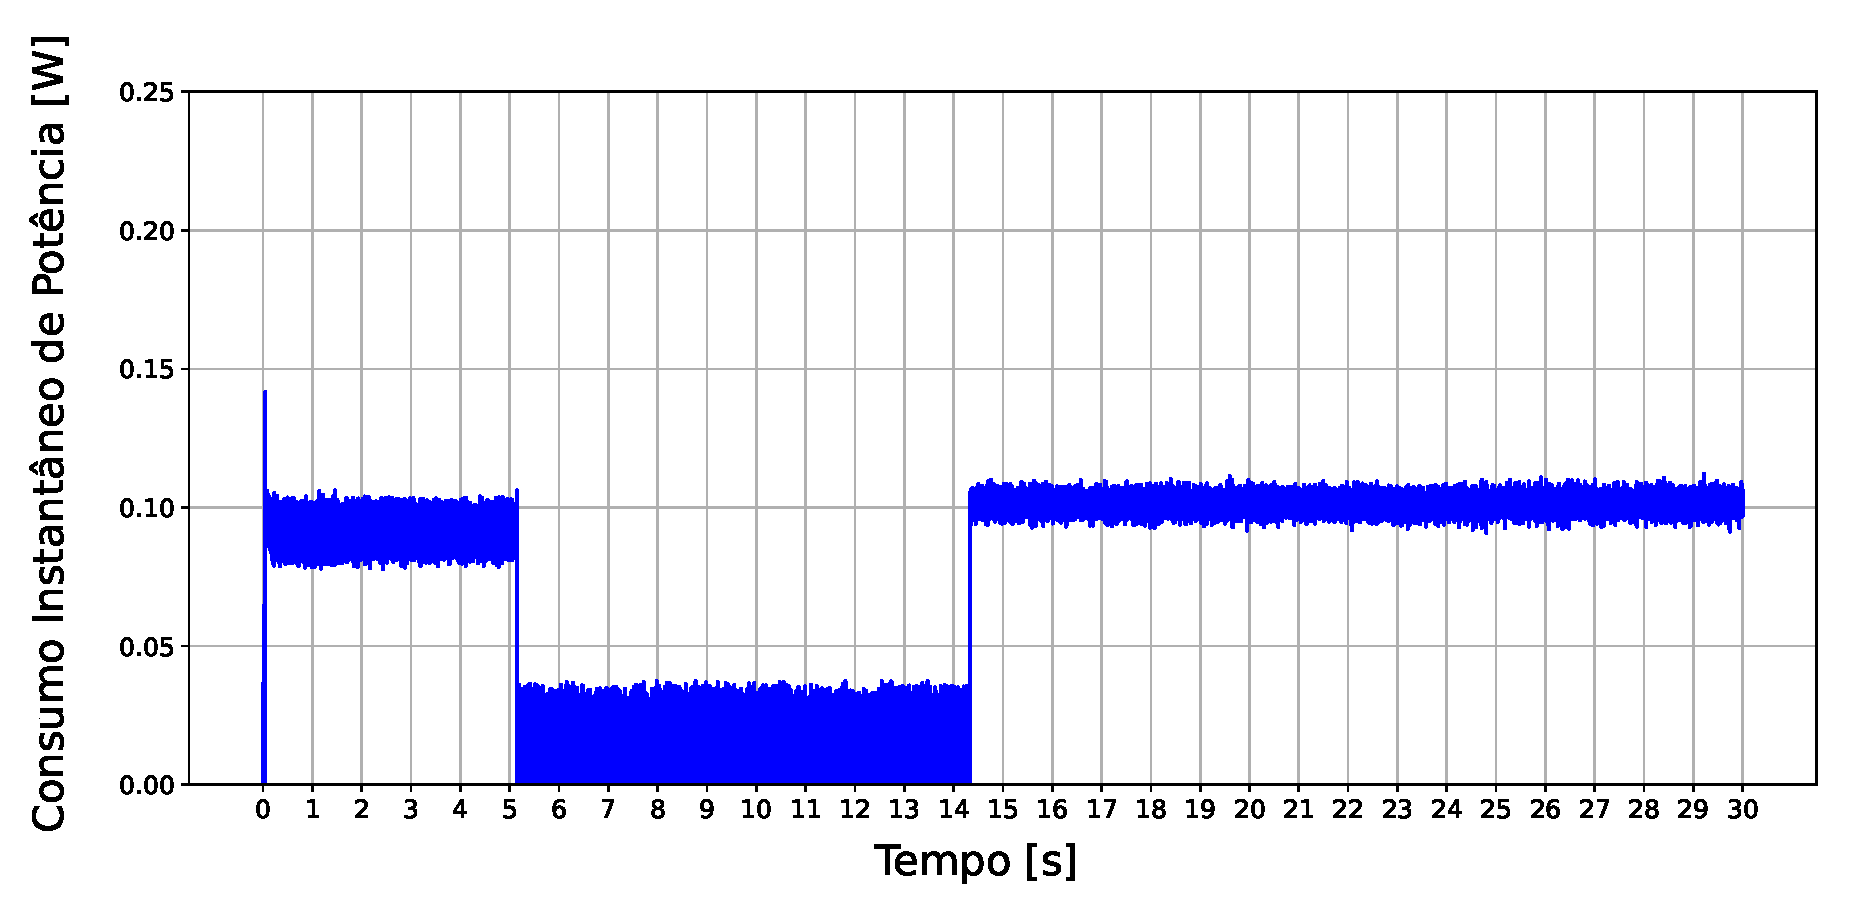
\includegraphics[width=1\linewidth]{imagens/low_power.eps}
    \caption{Sinal de potência em modo low power por 10 segundos, fonte: autor}
    \label{fig:low_power}
\end{figure}

\subsection{Pré-processamento}
Para captura da componente temporal dos dados utilizados como entrada no modelo é necessário um pré processamento numa janela de dados, extraindo cinco atributos de cada um dos três eixos do acelerômetro, como descrito em \cite{hyerarchical_ML}. São eles: soma de todos os valores, maior valor, menor valor, valor médio e por fim desvio padrão dos dados, gerando assim quinze parâmetros que são fornecidos como entradas para os modelos de aprendizado de máquina.

Objetivando medir o consumo desta tarefa foi escrita uma aplicação que apenas realiza esses cálculos repetidamente, sobre uma janela de 432 amostras, maior janela proposta. Executando esta aplicação, foi obtido o sinal de potência consumida visto na Figura \ref{fig:only_features}. Foi calculado o valor médio do instante oito segundos até 28 segundos, obtendo uma potência média de 92.1 mW. As oscilações observadas são geradas pela diversidade de instruções executadas, visto que instruções de desvio condicional e de operações de ponto flutuante utilizam áreas diferentes do processador.

\begin{figure}[!ht]
    \centering
    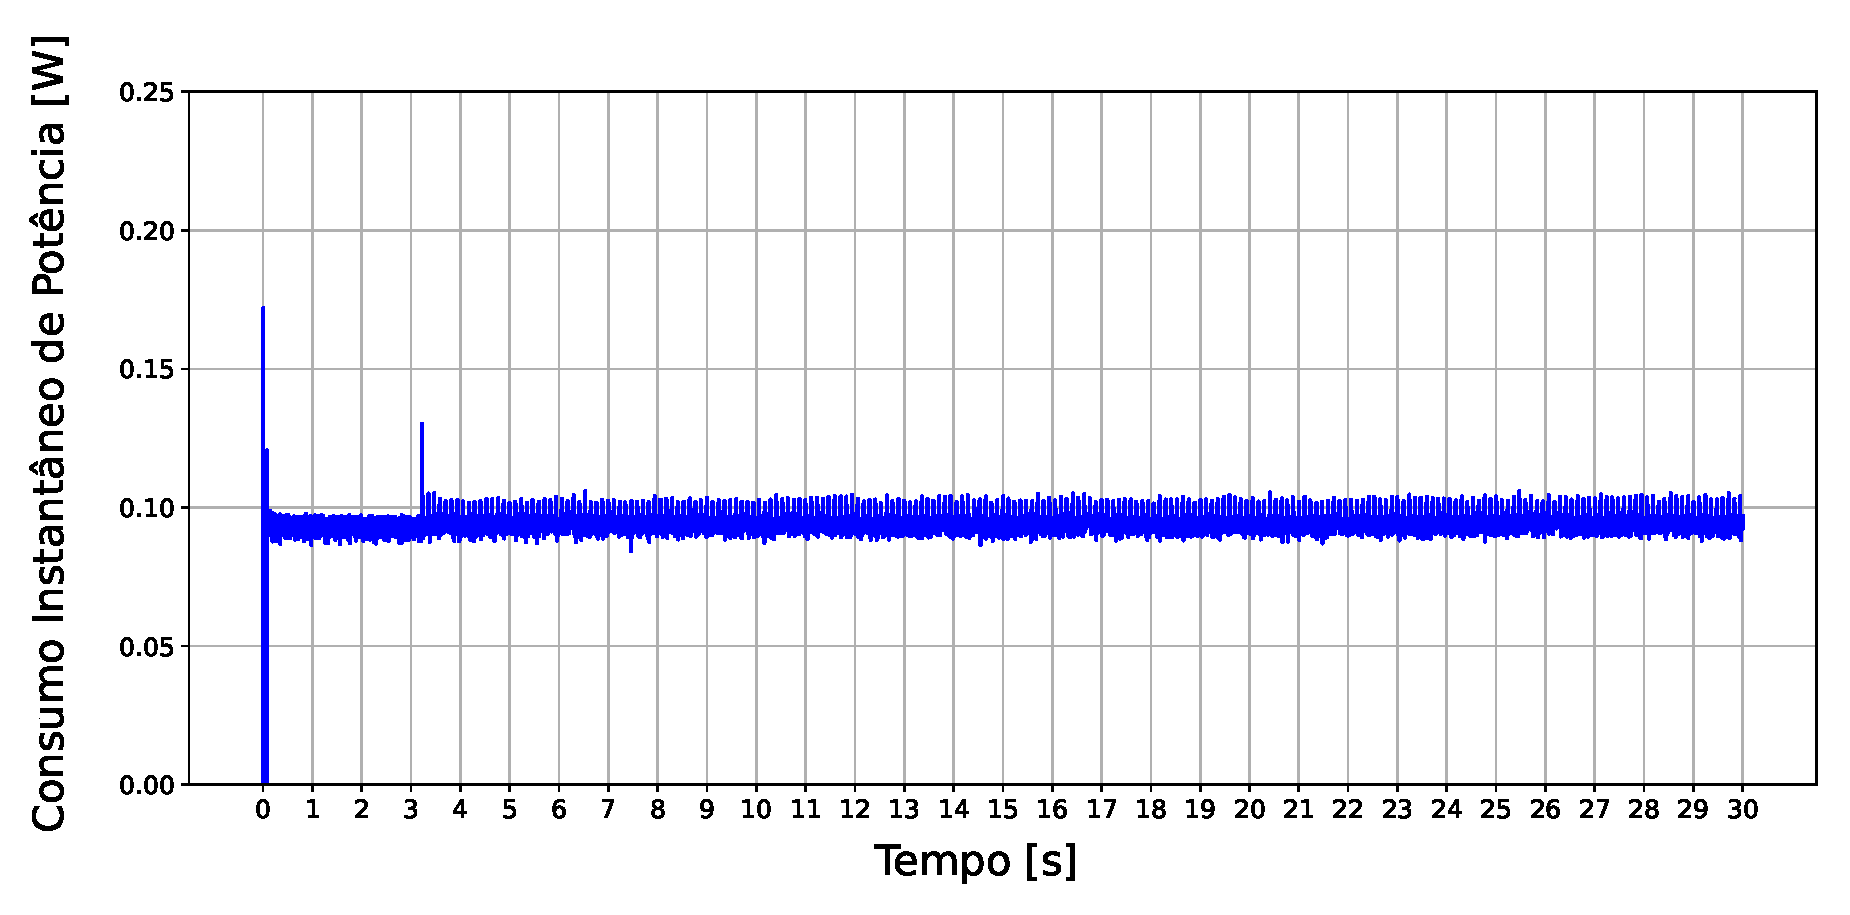
\includegraphics[width=1\linewidth]{imagens/only_features.eps}
    \caption{Sinal de potência somente extraindo atributos, fonte: autor}
    \label{fig:only_features}
\end{figure}

\subsection{Inferência}
Considerando que os modelos de aprendizado de máquina utilizados são redes neurais e que as variações da aplicação proposta apenas alteram a quantidade total de instruções executadas, entende-se que a potência média consumida durante a execução de uma inferência é comum a todos os modelos e a alteração do consumo energético vem exclusivamente da diferença dos tempos de execução. Portanto, para análise, são coletados dados de consumo durante a execução da inferência por um modelo. Foi escrita uma aplicação que, assim como a de extração de atributos, apenas executa o modelo repetidamente. Com isso foi obtido o sinal de potência visto na Figura \ref{fig:only_model}. O consumo instantâneo aqui se mantém aproximadamente constante, em torno de 106 mW, isso ocorre por as operações de ponto flutuante realizadas durante a execução do modelo somarem maioria das instruções executadas pelo processador.

\begin{figure}[!ht]
    \centering
    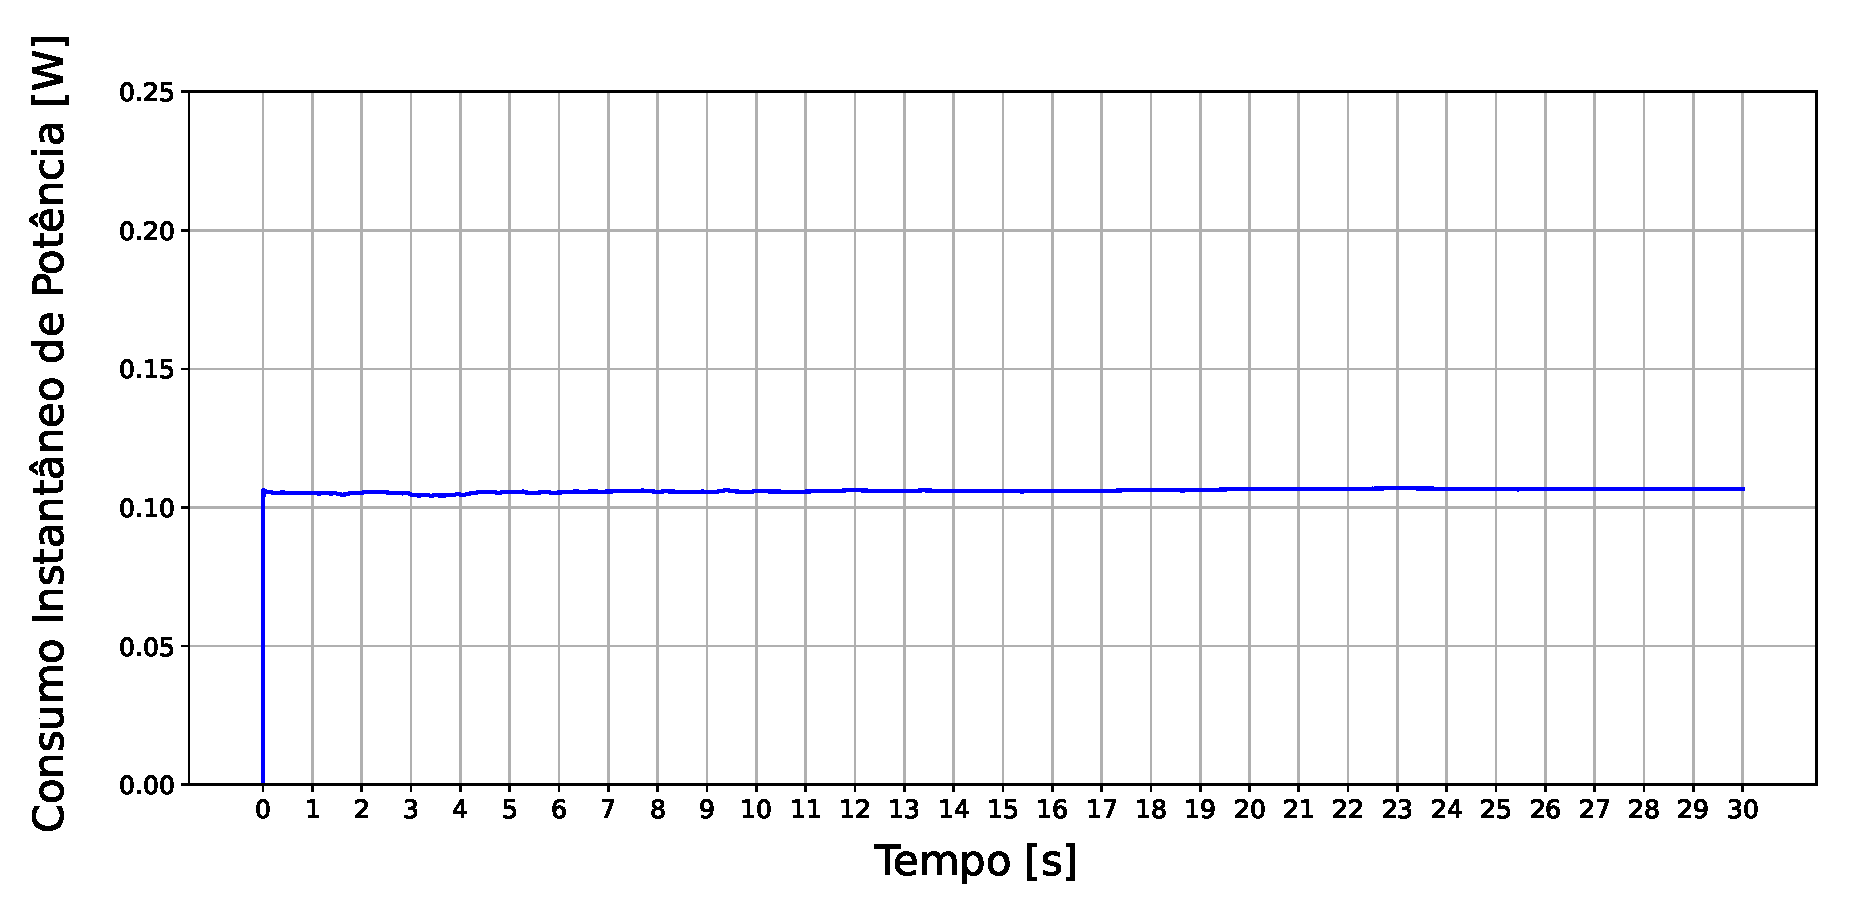
\includegraphics[width=1\linewidth]{imagens/only_model.eps}
    \caption{Sinal de potência somente realizando inferência, fonte: autor}
    \label{fig:only_model}
\end{figure}

\subsection{Transmissão}
Por fim, para aquisição da potência gasta durante uma transmissão de dados, foi utilizado o chip externo de Bluetooth, configurado como \textit{Broadcaster}, transmitindo doze bytes de dados a cada cinco segundos, resultando na Figura \ref{fig:beacon5s}. Os primeiros sete segundos correspondem a inicialização do processador e dos periféricos, podendo ser desconsiderado, pois estamos interessados apenas na transmissão. Portanto, considerando apenas a porção em regime permanente dos dados, de sete segundos até o fim, pode-se ver claramente cinco picos de consumo, com amplitudes proximas de 300 mW, com intervalos de cinco segundos entre si, resultando num valor médio de 231 mW ao longo de uma transmissão.

\begin{figure}[!ht]
    \centering
    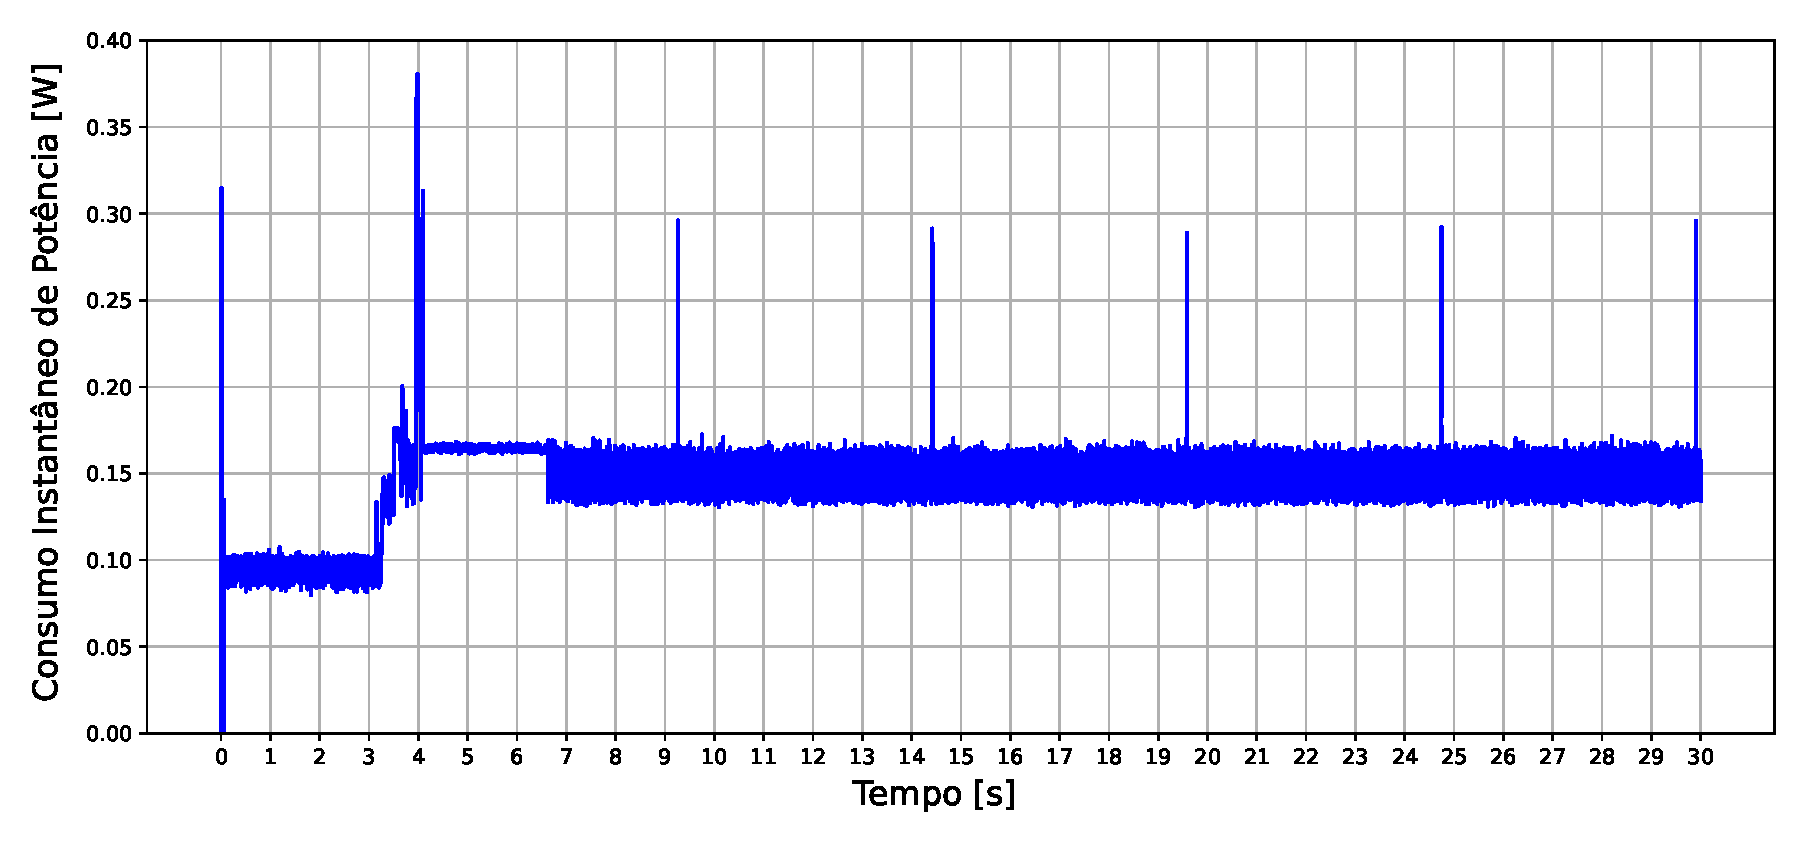
\includegraphics[width=1\linewidth]{imagens/beacon5s.eps}
    \caption{Sinal de potência coletado para o \textit{Broadcaster}, fonte: autor}
    \label{fig:beacon5s}
\end{figure}

\section{Dados de Tempo Coletados}
Além do consumo de potência durante a execução das tarefas, a descrição matemática necessita do tempo de execução destas tarefas. Para tal, foram escritas aplicações que executam diversas vezes um determinado modelo e reportam seu tempo de execução. Com destes dados em mãos foi extraída a média simples, resultando na Tabela \ref{tab:execution_times}.

\begin{table}[h]
    \centering
    \begin{tabular}{|c|c|}
         \hline Nome do Modelo  & Tempo de Execução [us] \\
         \hline 4:1             & 327                    \\
         \hline 4:2             & 367                    \\
         \hline 4:4             & 451                    \\
         \hline 4:8             & 615                    \\
         \hline 8:1             & 533                    \\
         \hline 8:2             & 645                    \\
         \hline 8:4             & 869                    \\
         \hline 8:8             & 1316                   \\
         \hline 16:1            & 1067                   \\
         \hline 16:2            & 1444                   \\
         \hline 16:4            & 2222                   \\
         \hline 16:8            & 3750                   \\
         \hline 32:1            & 2648                   \\
         \hline 32:2            & 4081                   \\
         \hline 32:4            & 6955                   \\
         \hline 32:8            & 12719                  \\
         \hline 64:1            & 7879                   \\
         \hline 64:2            & 13453                  \\
         \hline 64:4            & 24646                  \\
         \hline 64:8            & 47046                  \\   
         \hline
    \end{tabular}
    \caption{Tempo de execução em microssegundos para os modelos com 4 neurônios por camada}
    \label{tab:execution_times}
\end{table}


Foi escrita também uma aplicação para determinar o tempo de execução da função de extração de atributos. Extraindo a média dos tempos reportados temos a Tabela \ref{tab:getfeat_time}.

\begin{table}[h]
    \centering
    \begin{tabular}{|c|c|c|c|c|c|}
         \hline Tamanho da Janela [amostras] & Tempo [us]   \\
         \hline 54                           & 1507         \\
         \hline 108                          & 2926         \\
         \hline 216                          & 5785         \\
         \hline 432                          & 11600        \\
         \hline        
    \end{tabular}
    \caption{Tempo de execução para extração de atributos para diferentes tamanhos de janela}
    \label{tab:getfeat_time}
\end{table}

Por fim, o tempo tomado para realização de uma transmissão foi extraído dos experimentos realizados com o analisador de potência CC. Considerando que uma transmissão dura na média 25 amostras e sabendo que intervalo de amostragem é 0.1024 milissegundos, calculamos o tempo de transmissão como:
\begin{equation}
    t_{\text{tx}} = 25 \cdot 0.0001024 = 0.00256 \text{ segundos}
\end{equation}
    
% ---
% Resultados [ FEITO, REVISADO ]
% ---
\chapter{Resultados}
Como o objetivo deste trabalho é comparar duas aplicações, utilizamos a melhora percentual como figura de mérito, definida como:
\begin{equation}
    I = \frac{|{E_{base} - E_{prop}}|}{E_{base}} \cdot 100\%.
\end{equation}

\section{Análise}

De posse dos modelos matemáticos, dados coletados e utilizando a linguagem Python, foi construída um conjunto de funções para auxílio na análise dos dados. Inicia-se observando um intervalo de operação completo da aplicação proposta, conjuntamente com o da aplicação base, na Figura \ref{fig:compare_cycles}

\begin{figure}[!ht]
    \centering
    \includegraphics[width=1\linewidth]{imagens/compare_cycles.eps}
    \caption{Comparativo entre aplicação base para janela de 54 amostras e intervalo de transmissão de 0.1 segundos, fonte: autor}
    \label{fig:compare_cycles}
\end{figure}

Ampliando o final do intervalo de operação, na Figura \ref{fig:compare_cycles_zoom}, pode-ser ver em detalhes a transição de modo low power para a extração de atributos, execução e inferência e por fim a transmissão.

\begin{figure}[!ht]
    \centering
    \includegraphics[width=1\linewidth]{imagens/compare_cycles_zoom.eps}
    \caption{Ampliação no final do ciclo, fonte: autor}
    \label{fig:compare_cycles_zoom}
\end{figure}

\subsection{Variação do Modelo}
Para as combinações possíveis dos parâmetros descritos no início deste capítulo foram determinadas as melhoras percentuais na eficiência. Nota-se, na Figura \ref{fig:compare_datawindow}, que para janelas de dados com mais amostras há uma variação menor da melhora, pois o tempo decorrido em modo Low Power tende a dominar o total de energia consumido.

\begin{figure}[!ht]
    \centering
    \includegraphics[width=1\linewidth]{imagens/compare_datawindow.eps}
    \caption{Variação da profundidade do modelo e largura das camadas, fonte: autor}
    \label{fig:compare_datawindow}
\end{figure}

Na Figura \ref{fig:compare_tasks}, podemos ver o consumo da execução das diferentes tarefas para os modelos testados com janela de 54 amostras. Nota-se que o consumo total tanto para extração de atributos quanto para transmissão de dados é constante, com variações apenas na energia consumida na execução da inferência.

\begin{figure}[!ht]
    \centering
    \includegraphics[width=1\linewidth]{imagens/compare_tasks.eps}
    \caption{Variação da profundidade do modelo e largura das camadas, fonte: autor}
    \label{fig:compare_tasks}
\end{figure}

\subsection{Variação do Intervalo de Transmissão}
Por fim, é analisada quanto de melhora foi obtida para diferentes intervalos de transmissão da aplicação base. No gráfico da Figura \ref{fig:compare_intervals} são mostrados dois modelos por intervalo, aqueles com a maior e menor melhora para um determinado intervalo de transmissão. Percebe-se que para intervalos de transmissão maiores a melhora é pequena, ainda que significativa, próximo de 4\%. Isto ocorre por o termo de modo low power ter grande participação na energia total consumida e a plataforma escolhida não ter como alvo o uso neste modo. Este efeito seria menos proeminente em plataformas dedicadas a este tipo de aplicação, como será discutido no Capitulo 7.

\begin{figure}[!h]
    \centering
    \includegraphics[width=1\linewidth]{imagens/compare_intervals.eps}
    \caption{Melhora de eficiência obtida em função do intervalo de transmissão, para o melhor e pior caso, fonte: autor}
    \label{fig:compare_intervals}
\end{figure} 

% ---
% Conclusão. [ FEITO, REVISADO ]
% ---
\chapter{Conclusões e Recomendações}
Com a realização dos testes, processamento dos dados coletados e análise dos resultados obtidos, conclui-se que há redução de consumo em todos os casos avaliados, com melhoras significativas, faixa em torno de 35\%, para intervalo de transmissão de 0.1 segundos, e melhoras menos significativas, em torno de 4\% para intervalo de transmissão de 5 segundos.

Na análise referente aos intervalos de transmissão observa-se uma diminuição da melhora de eficiência com o aumento do intervalo, isso ocorre devido ao hardware escolhido, que consome na faixa de 6 mW quando em modo low power, valor considerado alto diante do que outros hardwares do mercado tem a oferecer. Em trabalhos futuros sugere-se o uso de harware construído especificamente para este propósito, como o Arduino Nano 33 BLE Sense, que conta com o SoC NINA-B306, da fabricante Nordic Semiconductor, e consome na casa dos 50 uW quando em modo low power \cite{nina_module}. 

% ---
% ----------------------------------------------------------
% Finaliza a parte no bookmark do PDF
% para que se inicie o bookmark na raiz
% e adiciona espaço de parte no Sumário
% ----------------------------------------------------------
\phantompart

% ----------------------------------------------------------
% ELEMENTOS PÓS-TEXTUAIS
% ----------------------------------------------------------
\postextual
% ----------------------------------------------------------

% ----------------------------------------------------------
% Referências bibliográficas
% ----------------------------------------------------------
\printbibliography

%---------------------------------------------------------------------
% INDICE REMISSIVO
%---------------------------------------------------------------------
\phantompart
\printindex
%---------------------------------------------------------------------
%--------------------------------------------------------

\end{document}
